\documentclass[11pt,a4paper,twoside]{article}
\usepackage{package/lmuthesis}

\prof{Prof.\ Dr.\ Heinrich Hu{\ss}mann}
\title{Automated UI Discovering for Web Application}
\author{Changkun Ou}
\email{hi@changkun.us}
\bearbeitungszeitraum{1.7.2018 bis 31.1.2019}
\betreuer{Malin Eiband and Dr. Daniel Buschek}
\aufgabenstellung{
    \begin{description}
        \item[Problem Statement] Under standing user behavior helps designer optimize 
        their product user experiences. At the same time, user benefits more productive 
        from it. Since user intents are elusive, changeable and sometimes even undetermined, 
        predict their behavior usually difficult and impoissible. In most cases, a user may 
        performs a series of wasted actions before reach an intent destination. 
        Nevertheless, user intents becomes clear step by step after performs a series of 
        actions in a given context. 
        \item[Scope of the Thesis] To tackle the aforementioned challenges, the objective of this thesis is to develop a system that tracking user actions within a website, 
        As a first step, literature review ...
        Based on the literature review, a intent model should be developed ...
        Then a system should implements the ...
        Nevertheless, user intents becomes clear step by step after performs a series of actions in a given context. 
        \item[Tasks] conduct a literature review to identify (research) question that simulates user input and predicts user ...
        \item[Requirements] asdfasdf
        \item[Keywords] asdfasdf
    \end{description}
}
\acknoledgement{
    Thansk to everyone.
}
\abstract{
    This is a abstract.
}

\begin{document}

\makecover
\makeaufgabenstellung
\makededication
\makeabstract
\maketoc


\section{Introduction}

\subsection{Origin of Clickstream Research}

The word "clickstream" first coined in 1995 \cite{friedman1995}, a media comments article 
introduces a novel concept of tracing cyberlife of users over the nowadays "Internet". 
Afterwards, people realized the potential danger and value of tracing cyberspace, which opens a
large discussion of clickstream influences, such as frequency based mining of clickstream \cite{brodwin1995},
privacy concerns \cite{reidenberg1996governing}, and database schema of such a time series data \cite{courtheoux2000database}.

Privacy discussion concludes collecting traces over net clearly offence the rights of users,
the practice violates the openness and transparency of a service to a user.
Serious criticism arise the tracing becomes a loss of democratic governance \cite{gindin1997lost}.

Technologies is not guilty. After years of discussion, positive opinion proposes the rules 
\cite{reidenberg1996governing} and regulations \cite{skok1999establishing} in cyberspace,
means of protecting information privacy in cyberspace transactions \cite{kang1997information},
and approaches to resolve conflicting international data privacy \cite{reidenberg1999resolving}.

Subsequently, bussiness man agilely responses to the concept and immediately initate 
commercial tracking of their customer to improving marketing affects \cite{novick1995}, 
customer service and precise advertisment\cite{reagle1999platform, bucklin2000sticky}, 
even measuring product success \cite{schonberg2000measuring}.

At the turn of this century, common reviews start accept the technology of clickstream,
clickstream data has confirmed by industrial practice, which opens a new era in 
customer service \cite{walsh2000internet}, most of website users start accept their click path data 
be aggregate analysed on the server side \cite{carr2000hypermediation}.

Clickstream data grows fast and becomes plentiful, researchers start convey the original concept of clickstream,
tracking customer selections, into various applications, such as usability testing \cite{Waterson:2002:LOW:506443.506602},
understanding social network sentiment \cite{Schneider:2009:UOS:1644893.1644899}, and developed visualizing
technique to better interpret clickstream data \cite{Waterson:2002:DTU:1556262.1556276}.

Analysis, reports and characterizing of clickstream gains its popularity, Mobasher et al. \cite{Mobasher:2001:EPB:502932.502935}
suggests personalize user based on association rule from their web usage data. Chatterjee et al. \cite{chatterjee2003modeling} 
first proposed E-commerce websites should use clickstream to tracking customer navigation pattern instead of essential choice, 
associating and binding products for observing responses of a customer.

\subsection{This thesis}

% 讨论 clickstream 的起源,讨论 clickstream 的影响,
% 为什么 clickstream 变得重要,为什么 clickstream 是一个值得研究的类别,
% clickstream 的价值都体现在哪些方面,以前的一些 clickstream 都有些什么内容。

% 大体上介绍本论文想要研究 clickstream 的内容,
% 这包括如何开展 clickstream 数据的搜集工作,搜集任务是什么,主要使用的方法,
% 以及得出的结论。根据这些结论,文章提出了一个客户端的插件,
% 能够在现代浏览器上支持这样的预测,
% 同时还进一步探讨了此项功能作为浏览器内建功能甚至浏览器 API 的可能性。

\cleardoublepage
\section{Related Works}
\label{ch:relate}

% - 讨论 client-side 的 clickstream 为什么值得研究,比较服务端搜集的 clickstream 产生的明显变化是什么。
% - 讨论现有的 client-side clickstream 研究分别是针对什么方向的,他们的结论主要是什么,都有什么样的改进空间。
% - 以前的 clickstream 只有类别级的分配模型,通过人工设计某个特定网站的马尔科夫模型来学习用户在不同类别之间的跳转概率。但当变为客户端后,数据变得更加充分,用户在一段时间内可能不局限于某个特定的网站,同时可能被其他网站干扰。

In this chapter, we discuss the former research that releats to our work, including
the existing approaches to clickstream behavior modeling, the evolution of information 
behavior theory regarding how it adapts to our digital world, as well as the 
most related recent advances regarding sequence learning.

\subsection{Clickstream Behavior Modeling}

Clickstream behavior research can be traced back to the year when the word ``clickstream''
was invented. Eearly clickstream behavior research studied the navigational behavior
of user \cite{mandese1995clickstreams, brodwin1995} and 
they binary classified clickstream based on the degree of linearity.

Mobasher et al. discovered the effective and scalable techniques \cite{Mobasher:2001:EPB:502932.502935} for Web personalization
by using association rules and built a recommondation system. Goldfrab invistigates \cite{goldfarb2002analyzing} 
the website choice behavior based on clickstream data and suggests that clickstream simulate company strategy changes.
Afterwards, 
Chatterjee et al. \cite{chatterjee2003modeling} first conduct 
the previous research regarding clickstream to an actual commercial website.
They found that clickstream represents an implication that dynamic advertising
based on customer clickstream history influence the future clickstream of the customer
and increase the interaction with the dynamic advertisement.
More techniquely, Ting et al. uses common sequences to find unexpected browsing behavior \cite{Ting:2005:UMF:1092358.1092469},
and then use their findings to improve website design. 

The most recent research evolved the approach of clickstream modeling,
Wang et al.\cite{Wang:2016:UCC:2858036.2858107} proposed a unsupervised appraoch to model clickstream without labeling.
Chi et al. proposed an analysis framework \cite{chi2017towards} for the general understanding of online information behavior
in a specific page. However, their framework only fits for server side collected clickstream other than a real user clickstream.
Then, Wang et al. \cite{Wang:2017:CUB:3127338.3068332} improved their unsupervised appraoch,
and summarized more approaches for clickstream behavior modeling that identifies span ad abuse
for a specific website. Park et al. models and detects a behavior change among student while learning 
based on Poisson process \cite{Park:2017:DCS:3027385.3027430} to
help improve online learning experience. Amo et al. \cite{amo2018learning} further visualizes search-stream
behavior based on student clickstream on a class, and Shimada et al. proves \cite{Shimada:2018:OCD:3170358.3170412}
online change detection while monitoring on student behavior is possible based on a sliding window.

Zaloudek gives an review on the comparasion \cite{mastersthesis} traditional method to model clickstream data,
then proposed a principle component analysis based method for a semi-supervised learning
of clickstream data, however their approach does not work well on clustering task, and 
the best performance is obtained by traditional multilayer perceptron algorithm.
Chandramohan and Ravindran then further investigate the neural approach on clicksteam mining \cite{N:2018:NAB:3152494.3152505},
they verified that complexy LSTM with Attention mechanism is able to capture whether a user
is intent to buy a product or not based on server side collected clickstream.
Surprisingly, Gundala and Spezzano \cite{Gundala:2018:RDH:3184558.3191644} simply use a Lasso
regression based on sofisticated feature engineering 
archived AOC score 0.769 for reader demand hyperlink prediction on Wikipedia clickstream dataset.

Kammenhuber et al. is the first study regarding client side clickstream \cite{Kammenhuber:2006:WSC:1177080.1177110}.
They proposed a finite-state Markov model that models user's search behavior on a level of
topic categories. Unfortunately their dataset are collected from network package traffic,
and did not consider the time a user spend in each page.


% 关于 assistent 的研究
% @article{lieberman1995letizia,
%   title={Letizia: An agent that assists web browsing},
%   author={Lieberman, Henry and others},
%   journal={IJCAI (1)},
%   volume={1995},
%   pages={924--929},
%   year={1995}
% }

\begin{figure}[H]
    \centering
    \includegraphics[width=0.55\textwidth]{figures/branching-and-backtracking}
    \caption{Parallel browsing behavior: branching phenomenon \cite{huang2010parallel}}
    \label{fig:backtrace}
\end{figure}

Liu et al. \cite{liu2010understanding} studied a specific user behavior on dwell time on web pages, and concluded that
Weibull distribution is the most appropriate distribution to characterize this behavior. 
Huang et al. \cite{huang2010parallel, huang2012no} further 
noticed the behavior of branching parallel browssing and backtracking browsing
behavior on modern browsers, as shown in Figure \ref{fig:backtrace}, 
and presented an frequent analysis for the distribution of these two behavior individually.

Unfortunately, as we discussed above, the existed research regarding clickstream 
behavior modeling are either server-side modeling for an individual client or 
individually modelized for client-side behaviors with limited information of clickstream,
which does not stands for a real user behavior. 
Besides, the existed approaches are based on self-constructed features, 
the property of Markov memoryless and etc. Though the most recent
approach use neural networks, their findings only applies to specific context.

From the point of view of user behavior, they 
neither unambiguously justifies the foundation of their model, 
nor providing a significative performance of their model.

We, in this thesis, serialize the client side chronologic URL sequences with combines all 
these individually studied phenomena including the branching and backtracking browser 
feature. With this chronologic URLs, we seek to model and understand the essential user 
behaviors patterns while browsing on the Web.

\subsection{Theory of Information Behavior on the Web}
\label{sec:info-seek}

The thesis relates to information behavior theory since it supports the foundation of our
user study. This subsection discusses how the theory was concluded and 
the principles of the theory that sustain our thesis.

Information behavior research encompasses intentional information seeking and 
unintentional information encounters, and the roots to information behavior 
theory relates to information needs and uses \cite{doi:10.1002/aris.2009.1440430114} 
that arose in the 1960s.

However, the concept of information seeking behavior, was coined in late 1981 
by Thomas Wilson \cite{wilson1981user}, and he tries to formalize the process or 
activities of a conscious effort while information needs 
and uses. Figure \ref{fig:wilson-info-seek} illustrate the model of information behavior 
was proposed.

\begin{figure}[H]
    \centering
    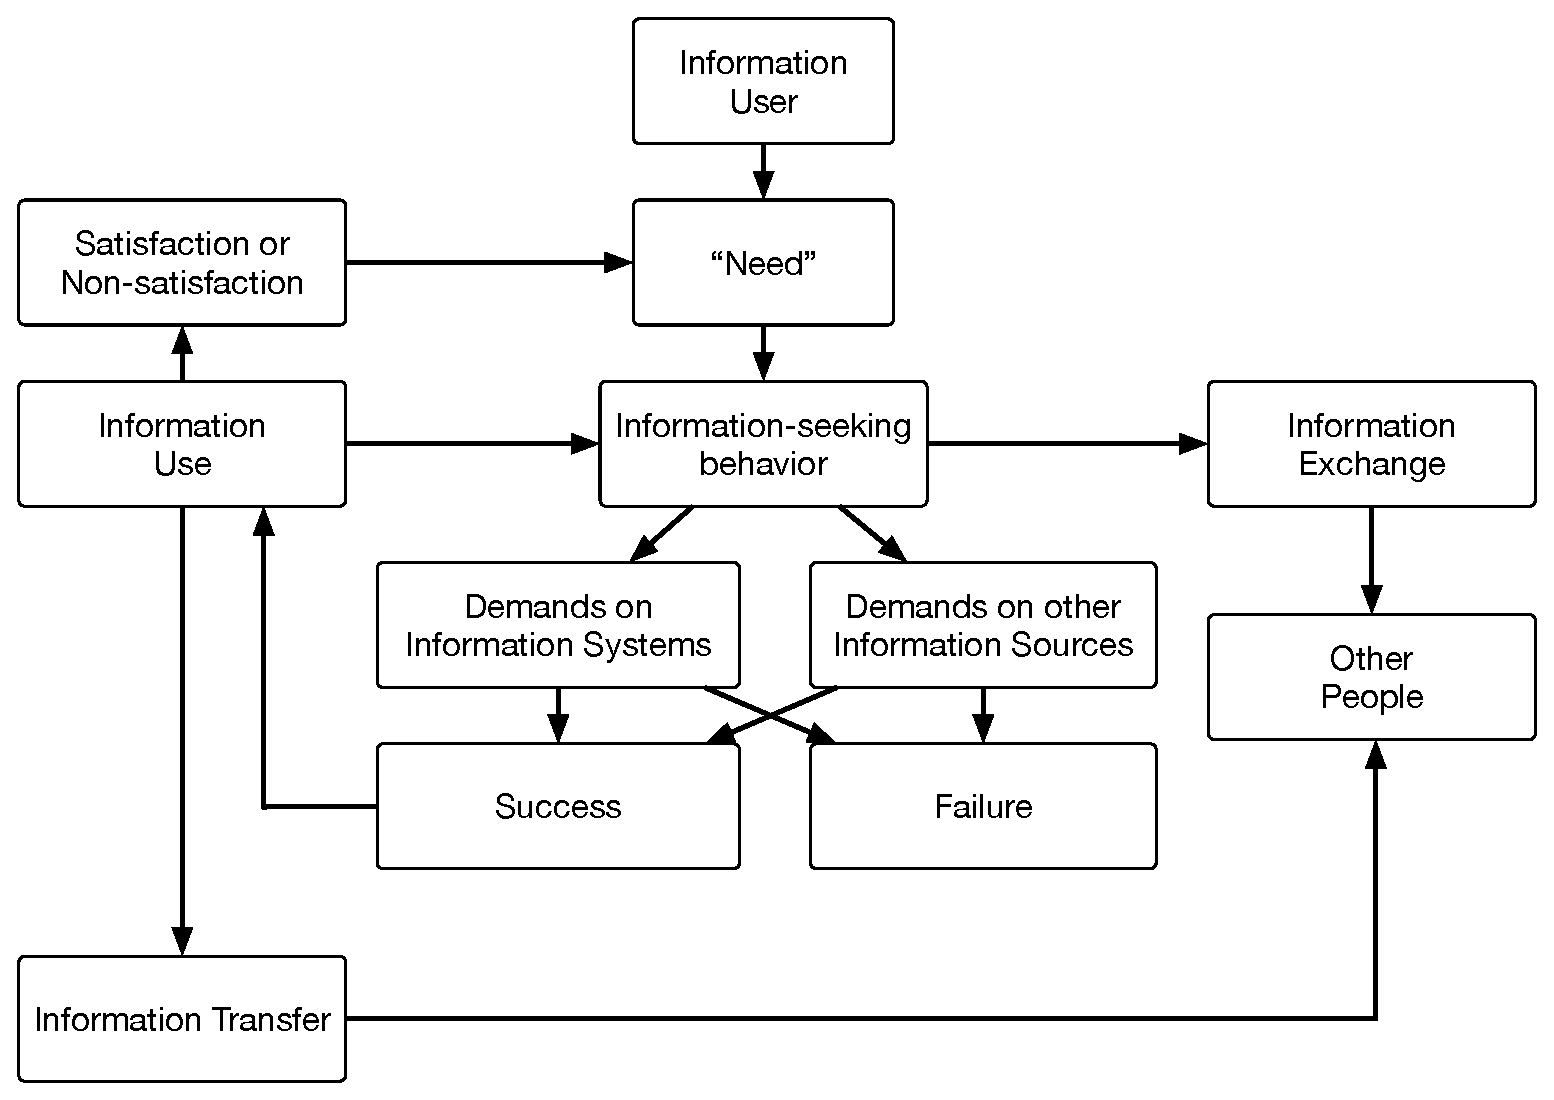
\includegraphics[width=0.7\textwidth]{figures/wilson-info-behavior}
    \caption{Wilson's information seeking behavior model \cite{wilson1981user}}
    \label{fig:wilson-info-seek}
\end{figure}

Wilson's model has been envolved many years since its origin, and it was revised 
and adapted to our digital world since the digital systems learns user preferences and 
changes \cite{giannini1998receiving} the way we receiving information.

David Ellis described a detailed group of activities for information seeking behavior \cite{ellis1989behavioural},
and then applied in physical and social science \cite{ellis1993comparison} and industrial
environment \cite{ellis1997modelling}.
In addition, his analysis was
based on grounded theory approach \cite{aceto1994grounded} and semi-structured interviews. 

Afterwards, Choo et al. adapts Ellis' Model and discussed \cite{choo1999information}
the information seeking behavior on the web through different activities rather 
than a single process, the applied activities are:
starting, chaining, browsing, differentiating, monitoring, and extracting.

``\emph{Starting}'' on the web indicates that a user identifies websites or pages
that containing the information of interests.
``\emph{Chaining}'' indicates that a user follows on starting page to other related pages.
``\emph{Browsing}'' then represents the activity that a user only skimming on the web
and quickly viewing the top-level informations. The ``\emph{differentiating}'' 
describes that a user on the web is selecting useful pages and choosing differentiated.
``\emph{Monitoring}'' activity is used for receiving updates on the sites, or revisit
the previously visited pages. Finally ``\emph{extracting}'' is the activity that a user
systematically extracts informations from a interested page or website.

By applying these activities, Choo et al concludes general user behaviors on the web are
undirected viewing, conditioned viewing, informal search and formal search.
Johnson further describes \cite{johnson2017patterns} seven more detailed behaviors 
patterns on the web, but did not given a working study that verify or prove their formation.

Although Wilson's model and Ellis' model are revised in recent works, however these improvements
are more generic and too complexy for describing user information behavior on the web.
Therefore, in this thesis, we only uses the an antecessor of Wilson's framework \cite{wilson1997information} and 
Ellis' model \cite{ellis1997modelling} to formalize and justify our lab study experiment later in Chapter \ref{ch:exp}, 
as a fundation of our work.

% \subsection{Theory of Sequence to Sequence Learning}

\cleardoublepage
\section{Literature Review}

TODO

\cleardoublepage
\input{contents/ch04-impl}
\input{contents/ch05-study}
\input{contents/ch06-conclusion}
\input{contents/ch07-future}
\part*{Appendix}
\appendix
\addcontentsline{toc}{part}{Appendix}
\fancyhead[LE,RO,LO,RE]{} % No headline on top of each page

All resources relates to the thesis are open source, 
they can be found publicly in:

\begin{itemize}
    \item Thesis homepage: \url{https://changkun.us/thesis/};
    \item GitHub repostory: \url{https://github.com/changkun/MasterThesisHCI/}.
\end{itemize}

All related text, picture and video content are licensed under a 
Creative Commons Attribution-NonCommercial-ShareAlike 4.0 International 
License\footnote{\url{http://creativecommons.org/licenses/by-nc-sa/4.0/}}.
The other parts of the thesis (such as program source code) are licensed 
under a MIT Public License
\footnote{\url{https://github.com/changkun/MasterThesisHCI/blob/master/LICENSE}}.

\section{Content of enclosed USB}
\label{appendix:a}

\begin{enumerate}
    \item $/documents/$ - TODO
\end{enumerate}


\section{Tasks and Questionnaire in Lab Study}
\label{appendix:b}

\subsection{Phase 1: Browsing Task}

This section approximately takes 80 minutes.

In this study, you are asked to accomplish a series of tasks provided in the table below.
Please read the following tips carefully before you do the task.

\begin{enumerate}
    \item \textbf{Please start from the given starting page.} You can then visit any other page. 
          For instance, if you find a task too difficult, you can visit any other websites 
          that help you accomplish the task (e.g. Google as a search engine), but you 
          should only use the browser.
    \item The tasks are designed to take \textbf{5~10 minutes}. Do not feel stressed if you spend 
          more time because you have 80 minutes in total to \textbf{do the 9 tasks}. You will 
          be notified if you spend more than 10 minutes on a task. You can decide to go to 
          the next task or spend some to accomplish the unfinished task. 
    \item \textbf{Close the browser before you start working on the next task.}
    \item \textbf{Unfortunately, questions cannot be answered while doing the tasks.
          Please ask them before starting a task if something is not clear. }
\end{enumerate}

\subsubsection{Task Group 1: Amazon.com}

\textbf{Task Category: Shopping}

\begin{enumerate}
    \item Assume your smartphone was broken and you have 1200 euros 
          as your budget. You want to buy an iPhone, a protection case, and a wireless 
          charging dock. Look for these items and add them to your cart.

          \textbf{Requirement to Finish}: Click ``Proceed to checkout'' when you finished, exit the browser when you see the ``sign in'' page.
    \item You want to buy a gift for your best friend as a birthday present.. Add three items to your cart.
    
          \textbf{Requirement to Finish}: Click ``Proceed to checkout'' when you finished, exit the browser when you see the ``sign in'' page.
    \item Look for a product category that you are interested in and start browsing. Add any items to your cart that you would like to buy. 
           
          \textbf{Requirement to Finish}: Clicked ``Proceed to checkout'' when time is up, exit the browser when you see the ``sign in'' page.
\end{enumerate}

\textbf{How difficult was the task? (1~5, 1 means very easy, 5 means very difficult)}

$\rule{1cm}{0.15mm}$, $\rule{1cm}{0.15mm}$, $\rule{1cm}{0.15mm}$

\subsubsection{Task Group 2: Medium.com}

\textbf{Task Category: Media}

\begin{enumerate}
    \item Assume you were making plans for your summer vacation. You want to visit Tokyo, Kyoto, and Osaka. 
          You want to find out what kind of experience other people made 
          when traveling to these three places in Japan. Your task is to find three posts 
          for traveling tips regarding these cities. Elevate a post if it is one of your choices.

          \textbf{Requirement to Finish}: Write down three tips.
          Close the browser when you are finished.

          \item Assume you got an occasion to visit China for business. You are free to travel to China for a week. 
          You want to make a travel plan for touring China within a week. Your task is to find out what kind 
          of experience other how people made when going to secondary cities or towns in China, then decide 
          on three cities you want to visit (excluding  Beijing, Shanghai, Guangzhou, and Shenzhen). 
          Elevate if a post helped you make a decision. 

          \textbf{Requirement to Finish}: Write down the names of the cities you decided. 
          Close the browser when you are finished.

    \item Visit a category you are interested in and elevate the post you like. 
    
          \textbf{Requirement to Finish}: Close the browser when time is up.
\end{enumerate}

\textbf{How difficult was the task? (1~5, 1 means very easy, 5 means very difficult)}

$\rule{1cm}{0.15mm}$, $\rule{1cm}{0.15mm}$, $\rule{1cm}{0.15mm}$

\subsubsection{Task Group 3: Dribbble.com}

\textbf{Task Category: Design}

\begin{enumerate}
    \item You are hired to a Cloud Computing startup company. You get an assignment to 
    designing the logo of the company. Search for existing logos for inspiration and 
    download three candidate logos you like the most.

    \textbf{Requirement to Finish}: Close the browser when you finished the download.

    \item You are preparing a presentation and need one picture for each of these animals: 
    cat, dog, and ant. Download the three pictures you like the most.

    \textbf{Requirement to Finish}: Close the browser when you finished the download.

    \item Explore dribbble and download images you like the most while you browse.
    
    \textbf{Requirement to Finish}: Close the browser when you finished the download.

\end{enumerate}

\textbf{How difficult was the task? (1~5, 1 means very easy, 5 means very difficult)}

$\rule{1cm}{0.15mm}$, $\rule{1cm}{0.15mm}$, $\rule{1cm}{0.15mm}$

\subsection{Phase 2: Questionnaire}

This section approximately takes 10 minutes.

\begin{enumerate}
    \item Age: $\rule{1cm}{0.15mm}$
    \item Gender: Female / Male
    \item What is your study program or occupation? 
    \item What are the websites that you access mostly? List your top-5 (max 10, including private use).
    \item What do you usually do  when you access these websites? Shortly answer your case for all the websites you listed in above and name  two common reasons, ordered by frequency.
    (For example, for YouTube, the most common reason could be ``Just for fun'', the second most common reason ``Looking for tutorial''. Then write as ``Mostly for fun, sometimes for learning'' below. )
    \item Do you use bookmarks to save webpages that you have found through a search engine? If so, why? 
    \item Which browser do you use mainly on your PC or Mac? 
          Chrome / Safari / IE / Microsoft Edge / Firefox / Others, the name is: $\rule{1cm}{0.15mm}$
    \item Would you like to participate in a follow-up study? The study will ask you to install a browser plugin for a week which anonymously records your browsing history. 
          Yes / No
    \item Do you have any feedback on this questionnaire?
\end{enumerate}

\subsection{Unselected Tasks}

\section{Raw Data Illustration}
\label{appendix:c}

\subsection{Subjective Difficulty Score from Lab Study}

\begin{table}[H]
      \small
      \centering
      \setlength{\belowcaptionskip}{10pt}
      \caption{Subjective task difficulty from lab study}

      \begin{tabular}{cccc}
            \toprule
            \textbf{Subject ID} & \textbf{Amazon.com} & \textbf{Medium.com} & \textbf{Dribbble.com} \\
            \hline
            1 & 2, 1, 2 & 2, 4, 1 & 2, 3, 2 \\
            2 & 2, 2, 1 & 2, 3, 1 & 1, 5, 1 \\
            3 & 3, 2, 2 & 2, 5, 3 & 3, 1, 3 \\
            4 & 3, 4, 2 & 2, 5, 2 & 3, 3, 2 \\
            5 & 2, 1, 3 & 3, 5, 3 & 2, 1, 3 \\
            6 & 2, 2, 1 & 3, 4, 1 & 1, 3, 2 \\
            7 & 3, 4, 2 & 3, 5, 3 & 4, 3, 2 \\
            8 & 1, 1, 1 & 3, 5, 2 & 2, 1, 1 \\
            9 & 2, 3, 2 & 2, 5, 2 & 3, 1, 1 \\
            10 & 1, 3, 2 & 2, 3, 2 & 2, 3, 3 \\
            11 & 2, 2, 3 & 1, 4, 5 & 1, 2, 3 \\
            12 & 3, 2, 1 & 3, 4, 1 & 3, 2, 2 \\
            13 & 4, 1, 3 & 5, 4, 2 & 2, 2, 1 \\
            14 & 2, 2, 2 & 2, 3, 1 & 2, 2, 1 \\
            15 & 5, 1, 3 & 2, 4, 1 & 4, 2, 3 \\
            16 & 1, 2, 1 & 1, 3, 1 & 1, 1, 1 \\
            17 & 3, 1, 1 & 3, 4, 3 & 2, 2, 3 \\
            18 & 2, 2, 1 & 2, 3, 1 & 3, 2, 2 \\
            19 & 3, 2, 2 & 2, 2, 1 & 1, 1, 2 \\
            20 & 1, 3, 2 & 3, 5, 1 & 2, 3, 2 \\
            21 & 3, 3, 2 & 3, 5, 4 & 2, 3, 5 \\
            \bottomrule
      \end{tabular}
      \label{table:diff}
\end{table}


TODO: add unselected tasks

\part*{Bibliography}

\addcontentsline{toc}{part}{Bibliography}
\nocite{*}
\bibliographystyle{plain}
\bibliography{literature/list}
\end{document}